Alle Komponenten der Applikation werden in jeweils einem Docker Container ausgeführt, um unabhängig vom Betriebssystem oder installierter Software (bis auf Docker) zu funktionieren. 
Damit die Container auch miteinander kommunizieren können, wurde im "docker-compose.yml" File ein Netzwerk namens "leoturnier" erstellt.

Das Frontend und Backend werden als Docker Image von einem Workflow auf Github Packages gepusht, welcher jedes Mal ausgeführt wird, wenn eine Änderung der Applikation auf Github gepusht wird.
Die Docker Images werden mit "Dockerfiles" gebaut. 

\section{Backend}

Das Dockerfile, das für das Docker Image des Backends benutzt wird, wurde von Quarkus automatisch generiert und sieht folgendermaßen aus. 

\begin{figure}[H]
    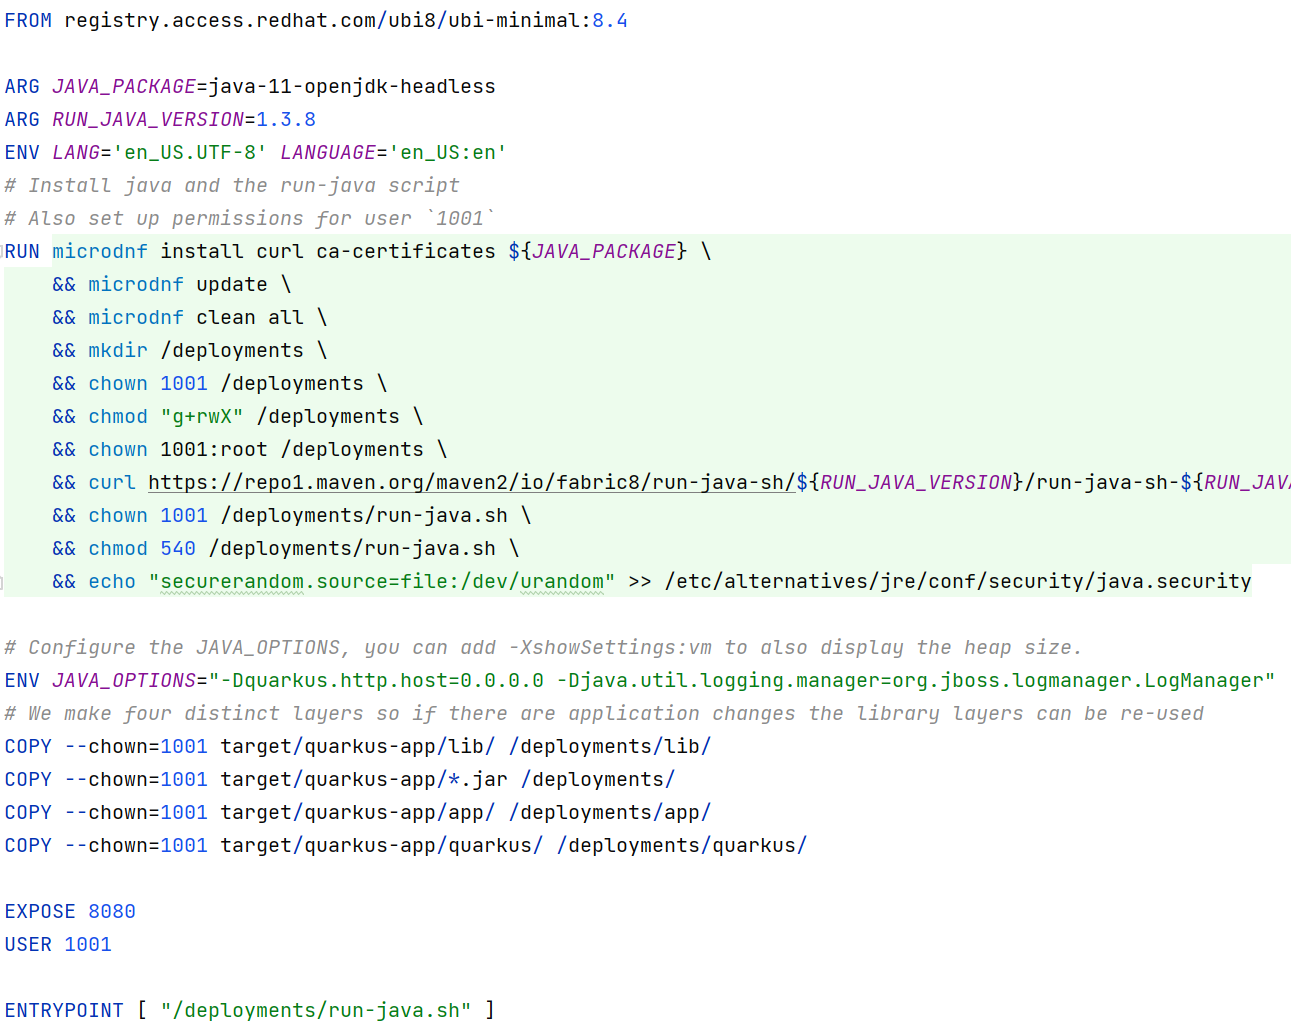
\includegraphics[scale=0.44]{pics/docker/dockerfile_backend.png}
    \caption{Dockerfile Backend}
\end{figure}

Im Grunde wird hier nur Java installiert und die für die Applikation wichtigen Files und Directories aus dem Backend in das Image kopiert.

\section{Frontend}
\setauthor{Benjamin Ecker}

Das Dockerfile, das für das Docker Images des Frontends benutz wird, enstand aus einer Vorlage eines bereits existierendes Dockerfile aus dem Internet \cite{deployment-dockerfile-1}.
Hier wird eigentlich nichts anderes gemacht, als Node und Nginx herunterladen um alle Libraries zu installieren, sowie alle wichtigen Files für die Angular App in das Image zu kopieren.
Die einzige Änderung die gemacht werden musste, war die Einbindung des "nginx.conf" um das Routing in der Angular App zu ermöglichen.

\begin{figure}[H]
    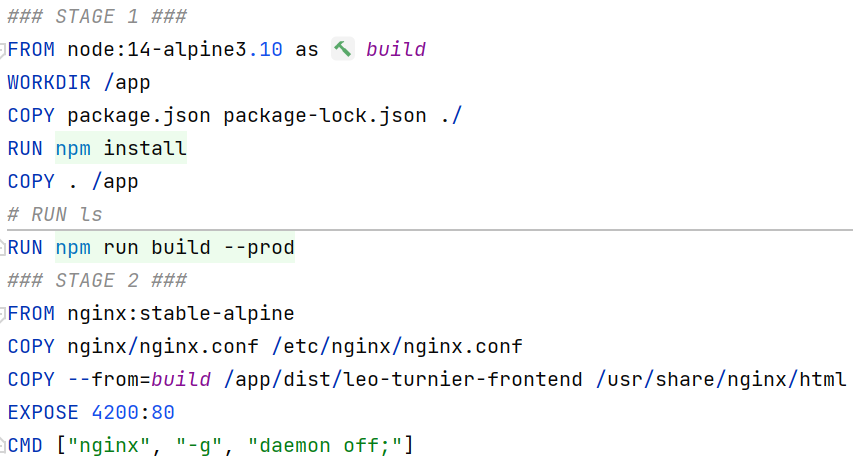
\includegraphics[scale=0.44]{pics/docker/dockerfile_frontend.png}
    \caption{Dockerfile Frontend}
\end{figure}

\section{Workflow}

Im Workflow wird dann die Registry angegebenen, in der die Images gepusht werden sollen, in dem Fall Github Packages, anschließend werden die Images gebaut und dann gepusht.

\begin{figure}[H]
    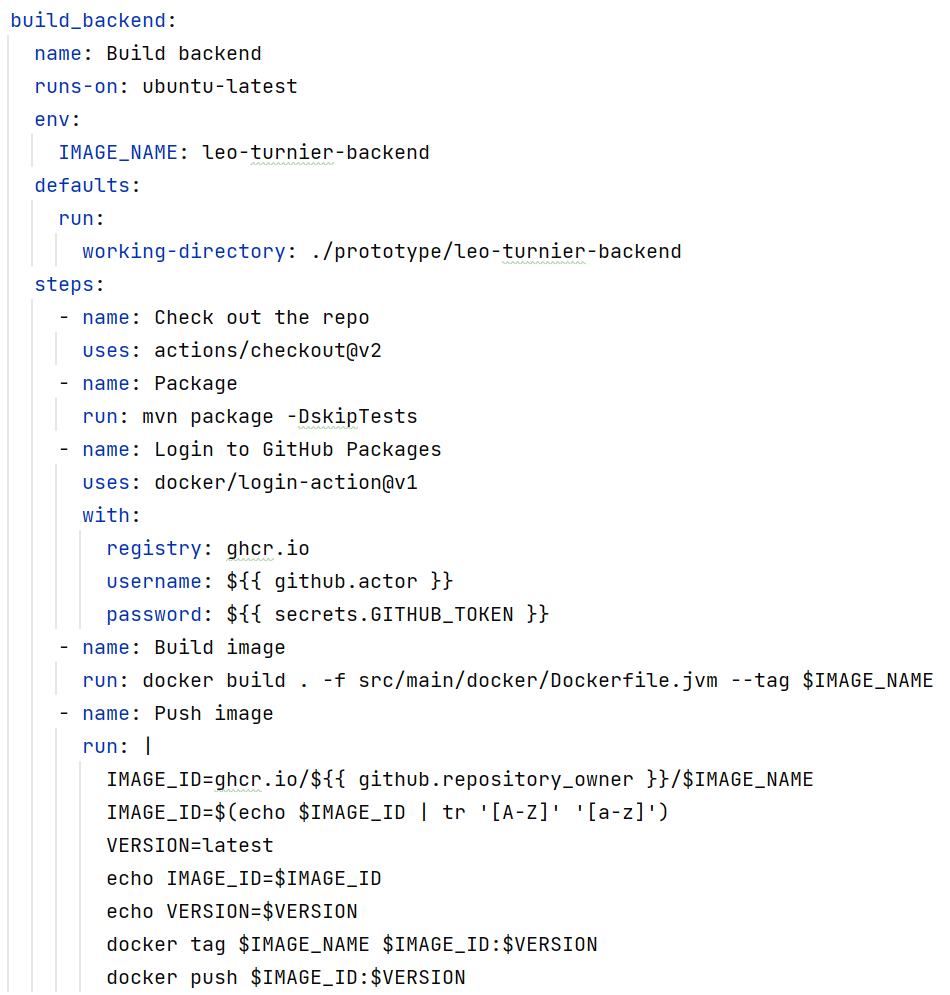
\includegraphics[scale=0.4]{pics/docker/workflow_backend.png}
    \caption{Workflow Backend}
\end{figure}

\begin{figure}[H]
    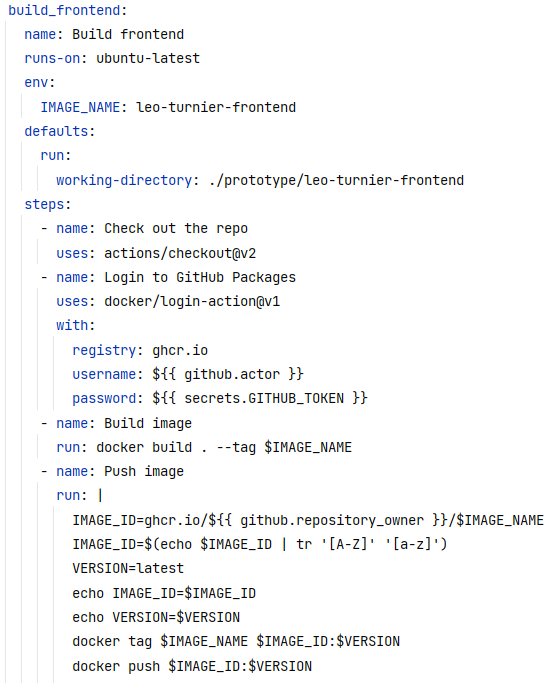
\includegraphics[scale=0.6]{pics/docker/workflow_frontend.png}
    \caption{Workflow Frontend}
\end{figure}

\section{Docker-Compose}

Ausgeführt werden die Images dann in einem Docker Container, der im dem "docker-compose.yml" File gestartet wird. 

\subsubsection{Backend}

\begin{figure}[H]
    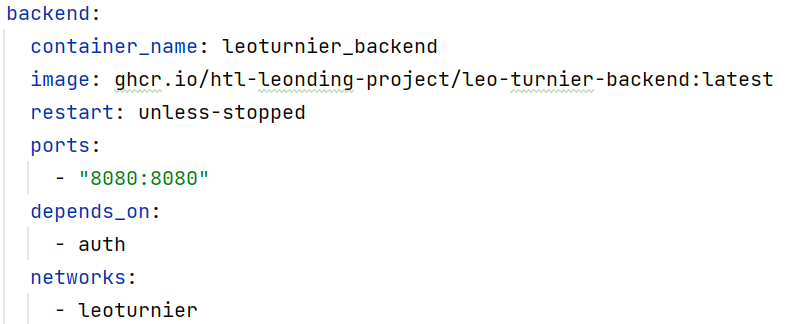
\includegraphics[scale=0.4]{pics/docker/docker-compose_backend.png}
    \caption{Docker Compose Backend}
\end{figure}

Hier wird das Docker Image, das im Vorhinein vom Workflow gepusht wurde, heruntergeladen und mit dem Port 8080 gestartet.

Zuvor wird noch die PostgreSQL Datenbank, in der die Turnierdaten gespeichert werden, gestartet.

\begin{figure}[H]
    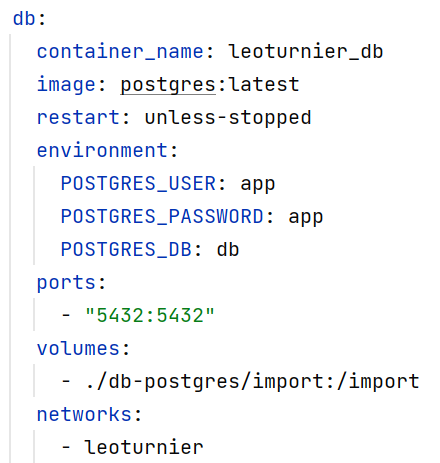
\includegraphics[scale=0.4]{pics/docker/docker-compose_db.png}
    \caption{Docker Compose Datenbank}
\end{figure}

\subsubsection{Frontend}

\begin{figure}[H]
    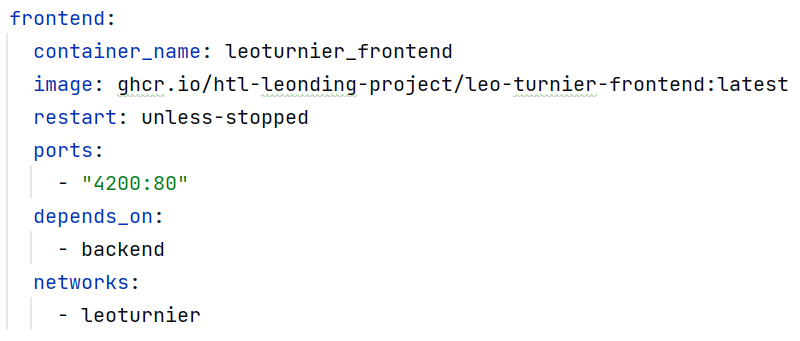
\includegraphics[scale=0.4]{pics/docker/docker-compose_frontend.png}
    \caption{Docker Compose Frontend}
\end{figure}

\subsubsection{KeyCloak}

Der KeyCloak Server sowie die Datenbank, in der die Userdaten verwaltet werden, werden ebenfalls im "docker-compose.yml" File gestartet.

\begin{figure}[H]
    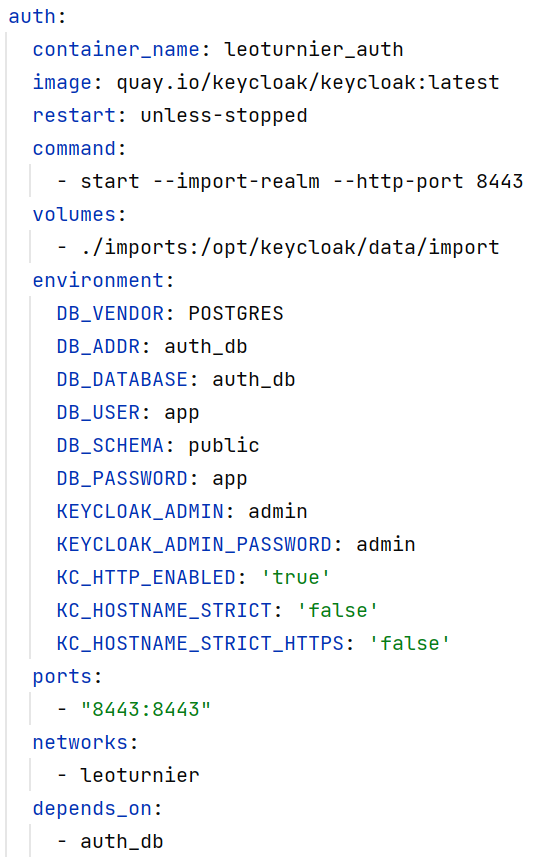
\includegraphics[scale=0.4]{pics/docker/docker-compose_auth.png}
    \caption{Docker Compose KeyCloak}
\end{figure}

Es werden die Konfigurationen importiert, der Port festgelegt, und User und Passwort für die verwendete Datenbank angegeben, welche zuvor ebenfalls im "docker-compose.yml" File gestartet wurde.

\begin{figure}[H]
    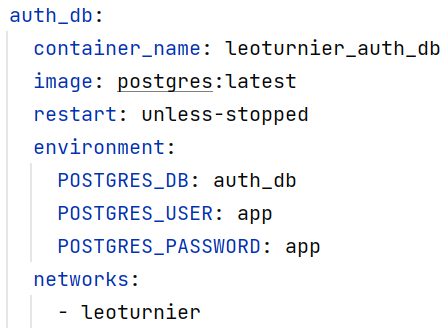
\includegraphics[scale=0.4]{pics/docker/docker-compose_auth_db.png}
    \caption{Docker Compose Userdatenbank}
\end{figure}